\subsection{Umfrage}
\label{ssec:konzept:client:umfrage}
Wie in Abb. \vref{fig:MockUmfrage} dargestellt, soll der Teilnehmer hier auf den zuvor erstellten Frageboge geleitet werden. 
Hier kann dieser diesen ausfüllen.
Die Fragen sollen dabei jeweiles in einer eigenen Karte angezeigt werden.
Über einen Button soll der Teilnehmer zur nächsten Frage weitergeleitet werden. 
Gleichzeigt soll der Benutzer eine Fortschrittsanzeige sehen können.
Zum Schluss der Umfrage soll der Teilnehmer diese mit einem Button beenden können.
Der Teilnehmer soll dabei Feedback erhalten, ob seine Teilnahme erfolgreich war. 

\begin{figure}[h]
	\centering
	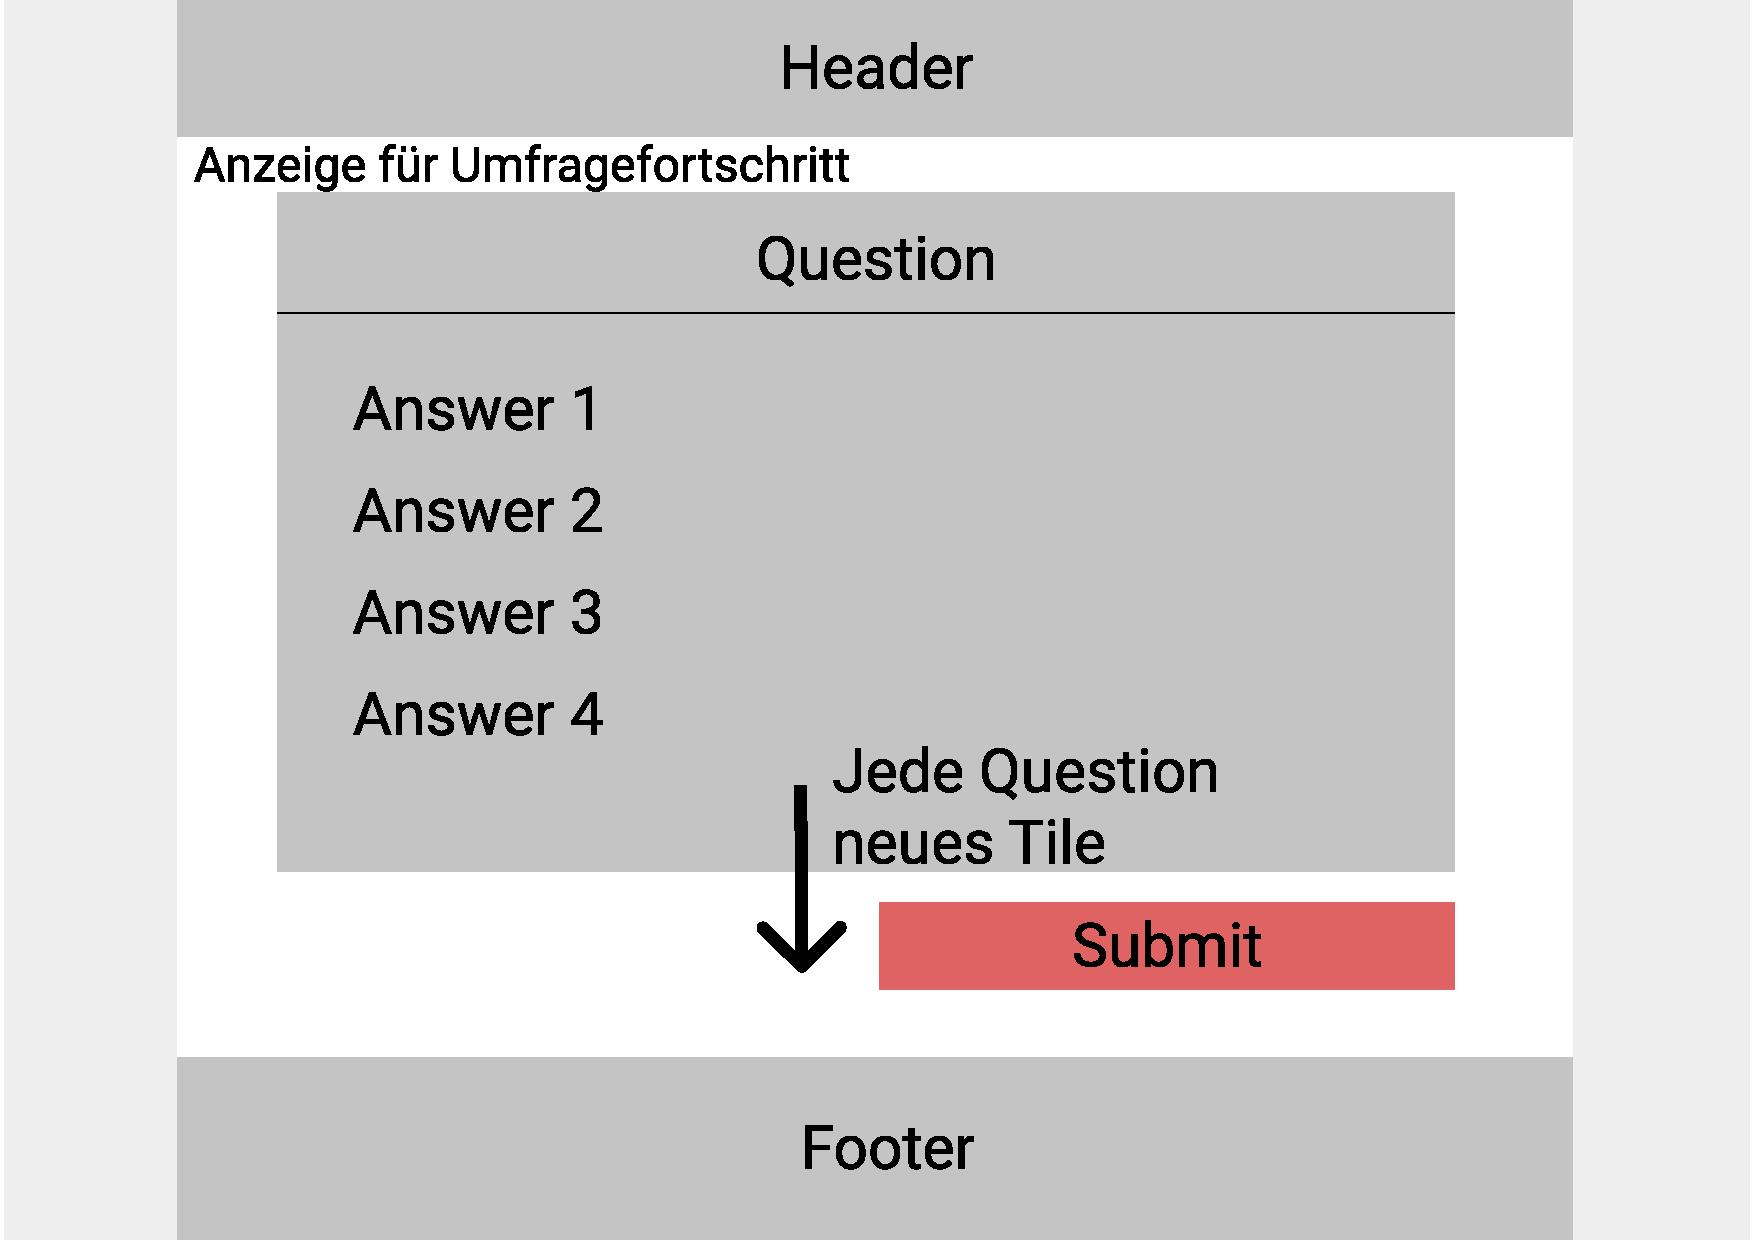
\includegraphics[width=0.7\textwidth]{img/konzeption/client/umfrage_teilnehmer}
	\captionsetup{justification=centering, format=plain}
	\caption[Mock-Up der Teilnahmeseite]{Mock-Up der Teilnahmeseite \\\figma}
	\label{fig:MockUmfrageTeilnehmer}
\end{figure}